\documentclass[a4paper,pagenum,english]{rnti}
\usepackage{graphicx}
\usepackage{listings}

\usepackage[T1]{fontenc}
\usepackage[latin1]{inputenc}
\usepackage{url}


\usepackage{xcolor}

\colorlet{punct}{red!60!black}
\definecolor{background}{HTML}{EEEEEE}
\definecolor{delim}{RGB}{20,105,176}
\colorlet{numb}{magenta!60!black}

\lstdefinelanguage{json}{
    basicstyle=\normalfont\ttfamily,
    numbers=left,
    numberstyle=\scriptsize,
    stepnumber=1,
    numbersep=8pt,
    showstringspaces=false,
    breaklines=true,
    frame=lines,
    backgroundcolor=\color{background},
    literate=
     *{0}{{{\color{numb}0}}}{1}
      {1}{{{\color{numb}1}}}{1}
      {2}{{{\color{numb}2}}}{1}
      {3}{{{\color{numb}3}}}{1}
      {4}{{{\color{numb}4}}}{1}
      {5}{{{\color{numb}5}}}{1}
      {6}{{{\color{numb}6}}}{1}
      {7}{{{\color{numb}7}}}{1}
      {8}{{{\color{numb}8}}}{1}
      {9}{{{\color{numb}9}}}{1}
      {:}{{{\color{punct}{:}}}}{1}
      {,}{{{\color{punct}{,}}}}{1}
      {\{}{{{\color{delim}{\{}}}}{1}
      {\}}{{{\color{delim}{\}}}}}{1}
      {[}{{{\color{delim}{[}}}}{1}
      {]}{{{\color{delim}{]}}}}{1},
}


\titrecourt{GeoCarteApp: A generic and personalized tool for the visualization of geospatial data}

\nomcourt{I. Bakerally et al.}


\titre{GeoCarteApp: A generic and personalized tool for the visualization of geospatial data}

\auteur{Noorani Bakerally\affil{1},
        Ghislain Atemezing\affil{2}\\
        Antoine Zimmermann\affil{1},
        Olivier Boissier\affil{1}}

\affiliation{
    \affil{1}Univ Lyon, MINES Saint-\'Etienne, CNRS, Laboratoire Hubert Curien UMR 5516, \\F-42023 Saint-\'Etienne, France\\
          \{prenom.nom\}@emse.fr\\
    %
    \affil{2}Mondeca, \\ 35 boulevard Strasbourg, Paris, France\\
          ghislain.atemezing@mondeca.com\\
          %\http{http://www.mondeca.com}
 }

%\resume{%
%
%}

\summary{GeoSpatial data is becoming more and more important in numerous domains. Many standards related to geospatial data such as GeoSPARQL or GML have been defined to facilitate interchange, reasoning and querying of geospatial data on the Web. However, there are still many datasets provided by organizations and open data portals which provide unstructured geospatial data. However, there is a need for such a tool which can help domain experts to bring different types of geospatial data, whether standardized, partially standard or heterogeneous data on a single map for analysis. In this paper, we provide a tool, GeoCarteApp, which can allow the visualization of geospatial data irrespective of the data model or format through the use of default or personalized configurations. We describe the tool, its features and show its usefulness for the trees' dataset related to Grenoble}

\begin{document}
\section{Introduction}
Currently, much data is available from open data portals. These data are encoded in different formats and based on different data models. Much of these data are geospatial data about different themes such as transportation, public services or tourism. These data are based on different data models, sometimes proprietary or sometimes standard. Due to the heterogeneity of geospatial data, map APIs (like Google Maps or MapBox) cannot directly consume the data for visualization purposes. As of now, map applications may directly consume data in GeoJSON, KML, ShapeFile and some others directly. For example, using Google Maps, one may drag and drop a GeoJSON data or text on a map and directly visualize the data. However, this is not yet directly possible for data in different formats and model like RDF, CSV, JSON etc. For example, the LinkedGeoData~\cite{stadler2012linkedgeodata} is a rich source of geospatial data which provides information collected by OpenStreetMap project and makes it available as RDF via their SPARQL endpoint \footnote{\url{http://linkedgeodata.org/sparql}} and RDF datasets. SPARQL queries can be written to obtain useful information from this source however the SPARQL results cannot be directly consume by map APIs for visualization. Same is the case for GeoNames or DBpedia and other rich sources of geospatial data. To allow the map application to consume data from heterogeneous sources, one has to programmatically parse the file and use the API to visualize the data on a map which can be a limitation for organization or domain experts not possessing the technical skills to do so.

This problem can be solved by using a generic approach which can allow data of different data models and formats to be automatically visualized on a map. In this paper, (1) we provide a description of the generic approach to generate a default visualization of geospatial data on a map in Section \ref{section:generic}, (2) we explain how this default visualization can be customized through configuration files to allow users to personalize the visualization according to their own preferences in Section \ref{section:customisation}, (3) we consider how this generic approach can help in case of Grenoble ....
\section{GeoCarteApp: A Generic Approach}\label{section:generic}

\begin{figure}
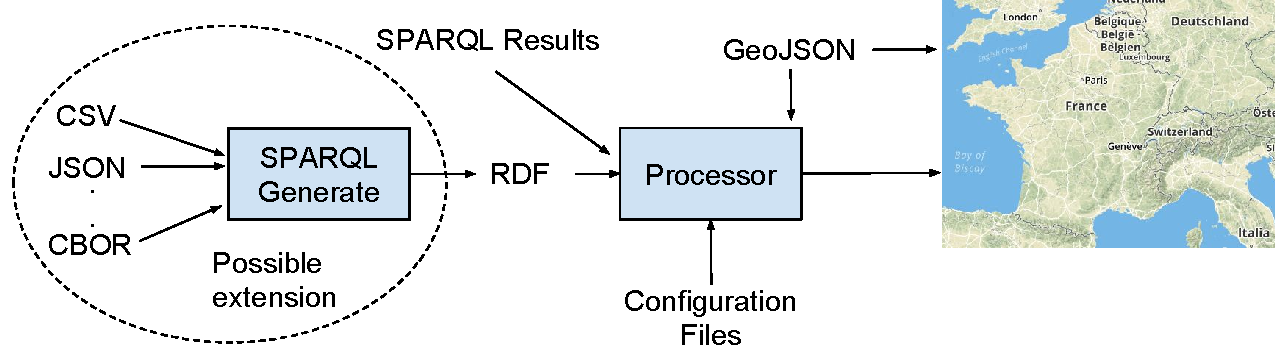
\includegraphics[scale=0.6]{img/generic_approach.pdf}
\caption{Generic Approach to visualize RDF Spatial data}
\label{fig:generic}
\end{figure}
Figure \ref{fig:generic} provides a high-level architecture of GeoCarteApp. The generic processor can consume geospatial data in RDF and produce a default visualization. A sample of this default visualization can be seen in Figure... 



As of now, the processor can only consume RDF. But it can be easily further enhanced by using SPARQL Generate \footnote{\url{http://ci.emse.fr/sparql-generate/} which produces RDF equivalents of data in other formats. These RDF equivalents can then be used as input to the generic processor.

The default visualization of RDF data is possible only due to standards like GeoSPARQL~[\cite{perry2012ogc}] and Linked Data best practices, like using the WGS84 vocabulary which is highly used by many datasets for encoding geographic coordinates~[\cite{schmachtenberg2014adoption}]. However, if these vocabularies are not used, it is still possible to visualize the data by using customized configurations.
  
  

\begin{lstlisting}[language=json,firstnumber=1, caption={Sample default configuration file}\label{listing:default_configuration}]
{"FranceGeoNames": {
	"dataSource": {
	"type": "RDFDataSource",
	"url": "http://www.geonames.org/3017382/about.rdf"
	}
},"Ecoles élementaires": {
	"dataSource": {
	"type": "GeoJSONDataSource",
	"url": "http://sig.grenoble.fr/opendata/Decoupage/json/DECOUPAGE_%C3%89L%C3%89MENTAIRES_EPSG4326.json"
	}
},"Arbres": {
	"latCol": "lat",
	"longCol": "long",
	"dataSource": {
	"type": "SPARQLDataSource",
	"url": "http://data.mondeca.com/egc2017/sparql",
	"query": "The SPARQL Query goes here"
}
}}
\end{lstlisting}
 
As shown in Listing \ref{listing:default_configuration}, to produce the default visualization, for RDF, the processor only needs the URL of the RDF file. It then follows GeoSPARQL and WGS84 vocabulary to extract the geospatial data. The processor can also consume SPARQL results. For the set of solutions from the SPARQL results, the column for the latitude and longitude should be specified. Like RDF, a GeoJSON file can stating its URL.


- default configuration file
- default configuration for RDF/SPARQL/GeoJSON
- default filtering mechanism
- default visualisation
	- unique colors
	- unique color for vectors


- Default Options
	- for each layer, there is a default unique color
	- a default description can be provided
		- where the popup include a popup with all the property and values for that layer
		



- Application can show:
	- RDF dataset
		- need to specify url of RDF dataset
		- by default it uses WGS84 ontology to identify latitude and longitude
		- as of now, works only for Marker layer
		- can be further generalised with GeoSPARQL ontology to other types of vector layer such as polygon,.. 
	- SPARQL Results
		- need to specify:
			- SPARQL endpoint
			- SPARQL Query
			- one solution for each marker
			- need to specify latitude and longitude
			- as of now, working only for Marke Layer

	- GeoJSON data by default
		- specify URL of GeoJSON file
		- works for both Marker and Vector Layer


\section{Customisation/Configuration (source)}\label{section:customisation}
- Default Options
	- for each layer, there is a default unique color
	- a default description can be provided
		- where the popup include a popup with all the property and values for that layer
	- Filters to be able to search for specific layers based on property and values
- Pop up data items:
	- key value pairs
	
	
Personalisation (Visualisation Part)
-------------------------------------
	- layer
		- derived attributes
		- specific customization for item with specific attribute
			- as of now, different icons for different markers having a particular attributes or attribute values
		- can customize the default desription and include in it property values of the layer
	- Marker
		- specify color
		- specify icon
	- constraints
		- area constraints
			- sometimes, not possible to show all markers
			- can specifiy section where the markers should be restricted
			- multiple sectors can be specified then, each marker is shown only if it is in all sections

	- filter labels

- as of now, no user interface to generate configuration, in an ideal situation, a user unaware of technicalities could use data from any source to generate map mashups


- labels 
- asssociate class names
- specify pop up data items
	- labels for different data items
- different types of constraints


\section{Application to Grenoble Data}\label{section:customisation}

\subsection{Transformation and Enrichment of Data}

\subsection{Transformation}
- ontologies used ?

\subsection{Enrichissement}
	- not yet ?
	- We added information about allergy-inducing trees from Wikipedia: https://fr.wikipedia.org/wiki/Liste_des_plantes_allergisantes
	

\section{Use Cases}
- search for trees which have to be diagnose
- specific icon for trees with allergies

PREFIX geo: <http://www.w3.org/2003/01/geo/wgs84_pos#>

SELECT ?tree ?genre ?level ?lat ?long
WHERE {
  ?tree geo:lat ?lat;
        geo:long ?long;.
  GRAPH <http://data.tree.com> {
    ?tree <http://data.lof.com/def/tonto#genreBotanique> ?genre .
    ?genre <http://data.lof.com/def/tonto#potentiel_allergisant> ?level }
  FILTER (?level > 3)
}

- others ?

- Species which can create allergies
- schools + hospital + allergy
- Species from DBPedia
- frequentation cible + allergy

\section{Recommendation on the Data}
% in French
Les données de localisation proposées dans ce défi souffrent du manque des métadonnées nécessaires pour faciliter leur exploitation, au moins sur deux aspects importants: le type de coordonnées géographiques et la correspondance des (X,Y) par rapport aux latitudes et longitudes. Ces éléments sont fondamentaux pour faciliter la réutilisation des données géographiques, surtout en qui concerne le positionnement et la meilleure interprétation des objets contenus dans les données. Il a fallu déterminer par des scripts ad hoc que les données géographiques utilisaient du EPSG:3945 (RGF 93/CC45) en limitant aux systèmes de coordonnées utilisées en France. 
De même, entre les différents fichiers il n’existe pas de relation “explicite” permettant de les relier entre elles, comme les clés dans les bases de données. Ce manque d’information nécessite un travail supplémentaire pour l’utilisateur des données de faire une inférence basée sur le même nombre de lignes dans les différents fichiers pour faire une corrélation de similarité basée sur les lignes.
Nous préconisons de mettre explicitation sur les métadonnées des informations de systèmes de coordonnées, ainsi que la mention de relations existantes entre les différents fichiers à exploiter par les utilisateurs. 

\section{Conclusion and Perspectives}
- the importance of a data model to describe data generically so that it can be used by map application
	- Perspective
		- enhance genericity
			- constraints ?
	- propose an ontology for such configuration
	- a definition of the processor to the processing of the dataset
	- a user interface to allow users to create their own configuration	
	- other data formats

\bibliographystyle{rnti}
\bibliography{biblioaz}

\end{document}
